\documentclass[letterpaper, reqno,11pt]{article}
\usepackage[margin=1.0in]{geometry}
\usepackage{color,latexsym,amsmath,amssymb,graphicx, float}
\usepackage{hyperref}

\hypersetup{
colorlinks=true,
linkcolor=magenta,
filecolor=magenta,
urlcolor=cyan,
}

\graphicspath{ {images/} }

\begin{document}
\pagenumbering{arabic}
\title{ELEC 481 Homework 4}
\date{02/06/22}
\author{Xander Naumenko}
\maketitle

{\noindent\bf Question 1.} Potential costs: 
\begin{itemize}
    \item Monetary cost for construction: there would be a large cost associated with the construction of the plant
    \item Monetary cost for maintenance: each years repairs must be made to ensure safety, plus the annual cost of fuel
    \item Cost of disposing nuclear waste: large societal (and monetary) cost to dispose of nuclear waste that doesn't decay for a very long time
\end{itemize}

Potential benefits: 
\begin{itemize}
    \item Cheaper power: power from nuclear plant can be much cheaper than the alternatives, such as solar or wind
    \item Better long term effects for the environment: if replacing coal/gas, much lower CO2 emissions which improves environmental effects
    \item Boosting local economy: construction of the plant creates jobs for local community
\end{itemize}

Stakeholder viewpoints: 
\begin{itemize}
    \item Locals: people who are close to the plant might object due to environmental/economic concerns
    \item Citizens who get power: people who get power from the plant (not necessarily locals) may appreciate the lower costs or have concerns about the implementation
    \item Indigenous people: the traditional indigenous land rights should be taken into account if applicable, and they should be consulted since they may have something valuable to say
\end{itemize}

{\noindent\bf Question 2.} Let $B$ be the PW of benefits and $C$ be the PW of costs. We are trying to solve the optimization problem $\frac{B}{C}$ subject to $B^2-18C+54=0$. Substituting these together we get that: 
\[
\frac{1}{18}\frac{\text d}{\text dB} \left( \frac{B}{B^2+54} \right) =0\implies \frac{B^2+54-2B^2}{(B^2+54)^2}=0\implies B=3\sqrt{3} 
.\]

Plugging this back into the limitation we find that $C=\frac{81}{18}=4.5$ and $\frac{C}{B}=1.155$. 

{\noindent\bf Question 3a.} Net benefits: 

\[
B_A=2400 (P/A, 0.09, 15)=A \frac{(1+i)^{n}-1}{i(1+i)^{n}}=\$19354.65
.\]
\[
B_B=5500 (P/A, 0.09, 15)=A \frac{(1+i)^{n}-1}{i(1+i)^{n}}=\$44333.79
.\]
\[
B_C=9600 (P/A, 0.09, 15)=A \frac{(1+i)^{n}-1}{i(1+i)^{n}}=\$77382.61
.\]
Net costs: 
\[
C_A=10000+1000 (P/A, 0.09, 15)-\frac{6000}{1.09^{15}}=\$16413.46
.\]
\[
C_B=17300+2750 (P/A, 0.09, 15)-\frac{4400}{1.09^{15}}=\$38258.93
.\]
\[
C_C=22000+6400 (P/A, 0.09, 15)-\frac{14000}{1.09^{15}}=\$69744.87
.\]
$B /C$ ratio: 
\[
B /C_A=1.179
.\]
\[
B /C_B=1.159
.\]
\[
B /C_C=1.110
.\]
Since A has the highest benefit over cost, it is the most efficient option (but may not earn the most overall). 

{\noindent\bf Question 3b.} Present worth: 
\[
PW_A=B_A-C_A=\$2941.19
.\]
\[
PW_B=B_B-C_B=\$6074.86
.\]
\[
PW_C=B_C-C_C=\$7637.74
.\]

Sine option C has the highest net present worth, it is the option that will result in the highest total benefit. 

{\noindent\bf Question 3c.} We can construct a spreadsheet with the given values as seen in figure \ref{fig:q3} for option A for example. Using the excel IRR we then get that: 
\[
IRR_A=13.0\%
.\]
\[
IRR_B=14.2\%
.\]
\[
IRR_C=13.7\%
.\]

\begin{figure}[htpb]
    \centering
    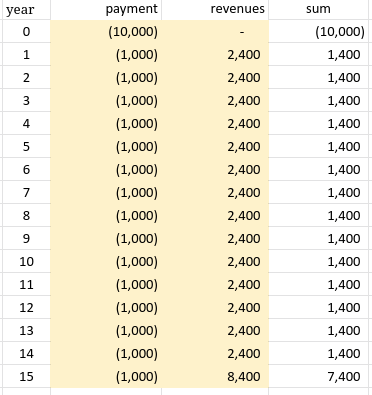
\includegraphics[width=0.8\textwidth]{q3}
    \caption{Income stream for project AA}
    \label{fig:q3}
\end{figure}

{\noindent\bf Question 3d.} Here we can simply take the total cost and divide by annual cost: 
\[
T_A=\frac{10000-6000}{2400-1000}=2.86\text{ years}
.\]
\[
T_B=\frac{17300-4400}{5500-2750}=4.69\text{ years}
.\]
\[
T_C=\frac{22000-14000}{9600-6400}=2.5\text{ years}
.\]

By this analysis option C is the best since it is the shortest. 

{\noindent\bf Question 4.} Break even interest rate is equivalent to the IRR, so using excel we can calculate that. The revenue stream is shown in figure \ref{fig:q4}, and using the IRR excel function we find that it is equal to 8.69\%. 

\begin{figure}[htpb]
    \centering
    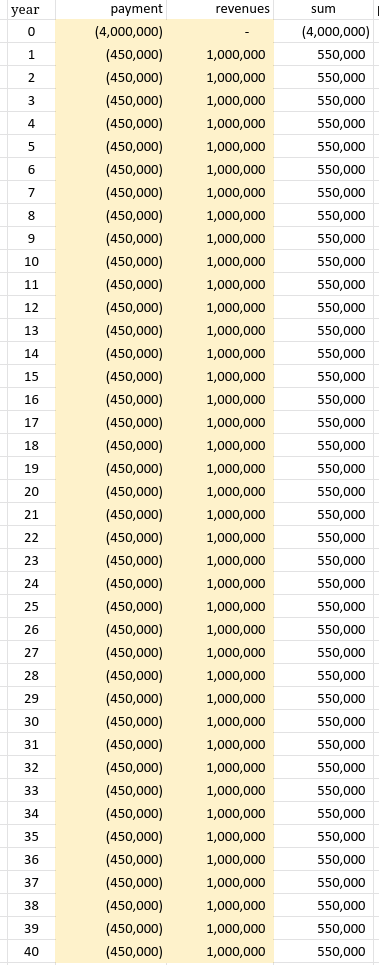
\includegraphics[width=0.8\textwidth]{q4}
    \caption{Revenue stream for question 4}
    \label{fig:q4}
\end{figure}


\end{document}
